\documentclass[fleqn,usenatbib]{mnras}
% MNRAS controls page geometry, body spacing and captions.
\usepackage[T1]{fontenc}
\usepackage{newtxtext,newtxmath}
\usepackage{amsmath,bm}
\usepackage{graphicx,booktabs,longtable,array,calc}
\usepackage[export]{adjustbox}
\usepackage{placeins,float}
\usepackage{xcolor}
\usepackage{bookmark}
\setlength{\emergencystretch}{2em}
\hypersetup{hypertexnames=false,colorlinks=true,linkcolor=blue!40!black,citecolor=blue!40!black,urlcolor=blue!40!black,pdftitle={Redshift evolution of the HI-weighted genus under Alcock-Paczynski distortions and foreground filtering}}
\providecommand{\tightlist}{\setlength{\itemsep}{0pt}\setlength{\parskip}{0pt}}
\newcommand{\pandocbounded}[1]{#1}
\DeclareRobustCommand{\todo}[1]{\textcolor{red!65!black}{\textbf{[TODO: }#1\textbf{]}}}

% Avoid artificial vertical stretching while retained wide figures float.
\raggedbottom
\XeTeXtracingfonts=0

\renewcommand{\thefigure}{S\arabic{figure}}
\renewcommand{\thetable}{S\arabic{table}}
\makeatletter
\newenvironment{suppfigure}{\par\noindent\begin{minipage}{\textwidth}\def\@captype{figure}\let\@makecaption\SFB@makefigurecaption\centering}{\end{minipage}\par}
\newenvironment{supptable}{\par\noindent\begin{minipage}{\textwidth}\def\@captype{table}\let\@makecaption\SFB@maketablecaption\centering}{\end{minipage}\par}
\makeatother
\begin{document}
\pagestyle{plain}
\onecolumn
\section*{Supplementary figures and area table}
These panels retain the full foreground and redshift comparisons underlying the compact main figures. Their statistics, curves and area values are unchanged from the saved v0.18 results. The regions describe normalized pipeline weights, not independently calibrated confidence levels.
\begin{suppfigure}\centering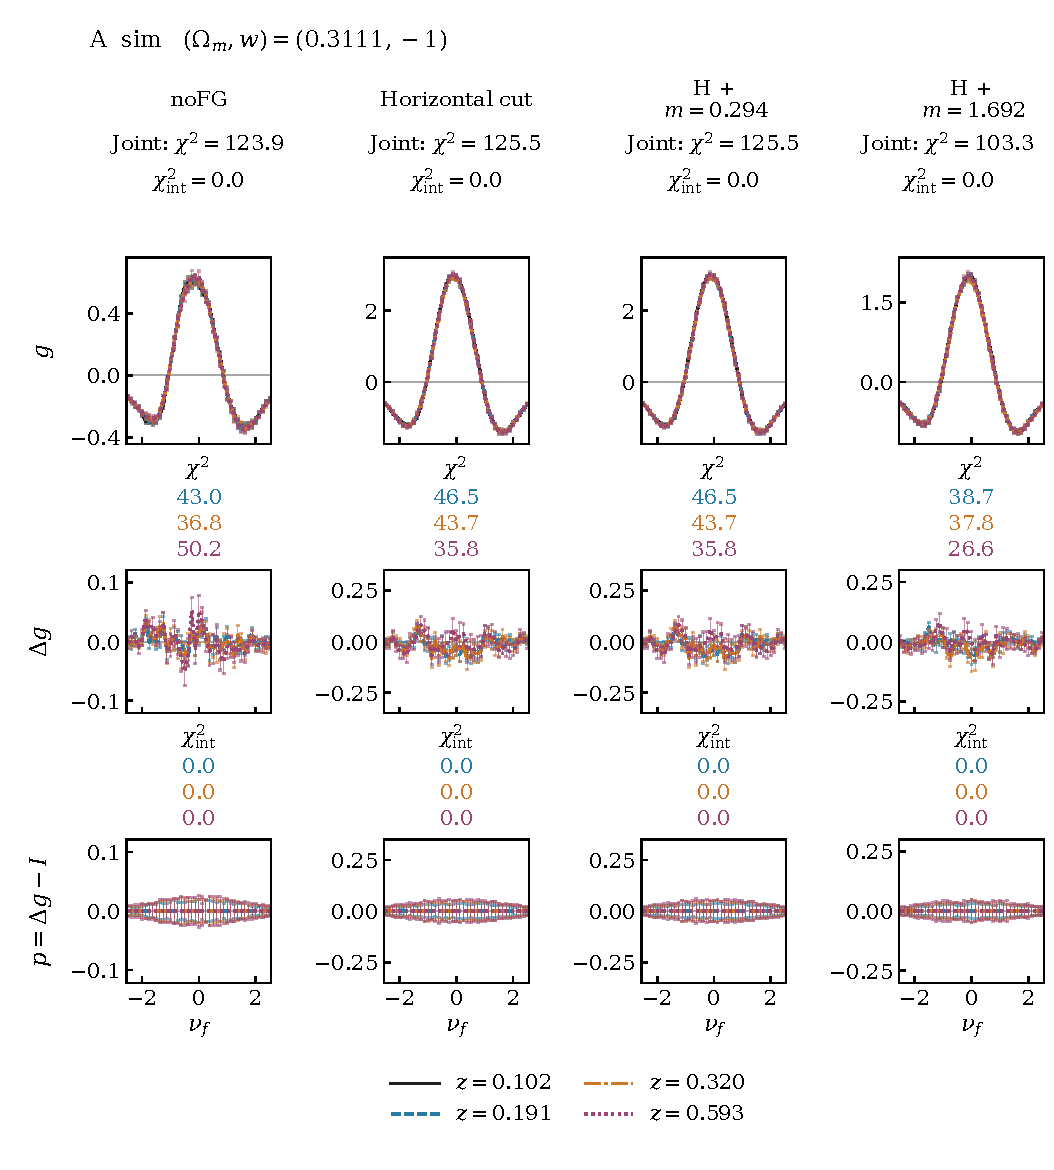
\includegraphics[page=1,width=.92\textwidth,height=.76\textheight,keepaspectratio]{figures/fig__cosmo_redshift_evolution.pdf}
\caption{Full genus, redshift differences and intrinsic-subtracted residuals for the simulation cosmology (A) and illustrative cosmologies (B and C, continued). All four foreground treatments are retained. Rows and error bars follow the main-text definitions.}
\end{suppfigure}
\clearpage
\begin{suppfigure}\centering\includegraphics[page=2,width=.92\textwidth,height=.76\textheight,keepaspectratio]{figures/fig__cosmo_redshift_evolution.pdf}
\contcaption{Panel B: $(\Omega_m,w)=(0.2,-1.4)$.}
\end{suppfigure}
\clearpage
\begin{suppfigure}\centering\includegraphics[page=3,width=.92\textwidth,height=.76\textheight,keepaspectratio]{figures/fig__cosmo_redshift_evolution.pdf}
\contcaption{Panel C: $(\Omega_m,w)=(0.42,-0.6)$.}
\end{suppfigure}
\clearpage
\begin{suppfigure}\centering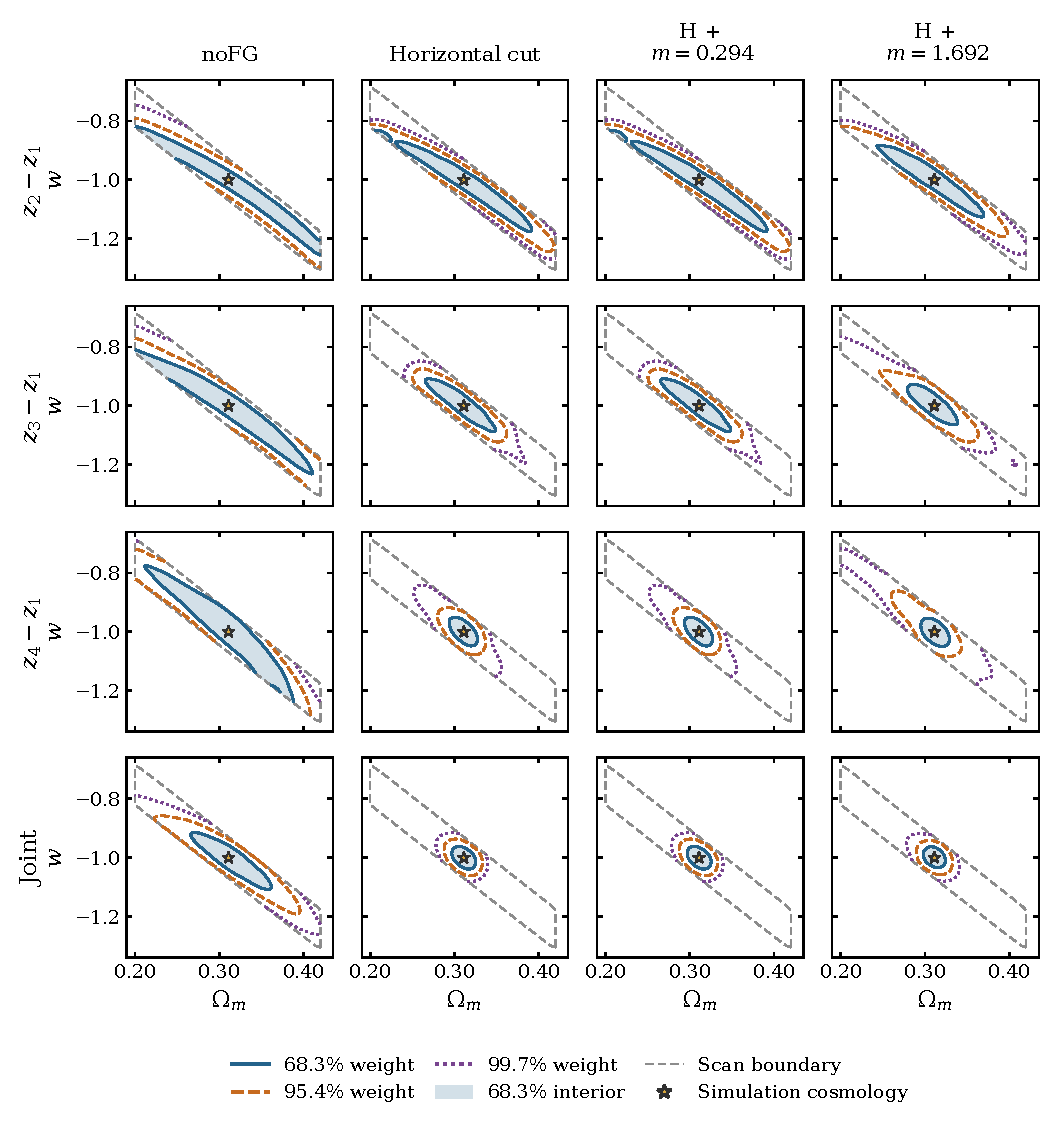
\includegraphics[width=.92\textwidth,height=.83\textheight,keepaspectratio]{figures/fig__intrinsic_subtracted_contours__four_cases_full.pdf}
\caption{All four foreground treatments, including the weak wedge, for the three redshift differences and joint statistic. Solid, dashed and dotted contours enclose 68.3, 95.4 and 99.7 per cent of the weight. Shading marks 68.3 per cent; grey dashed lines mark the domain boundary and stars the simulation cosmology.}
\end{suppfigure}
\clearpage
\begin{suppfigure}\centering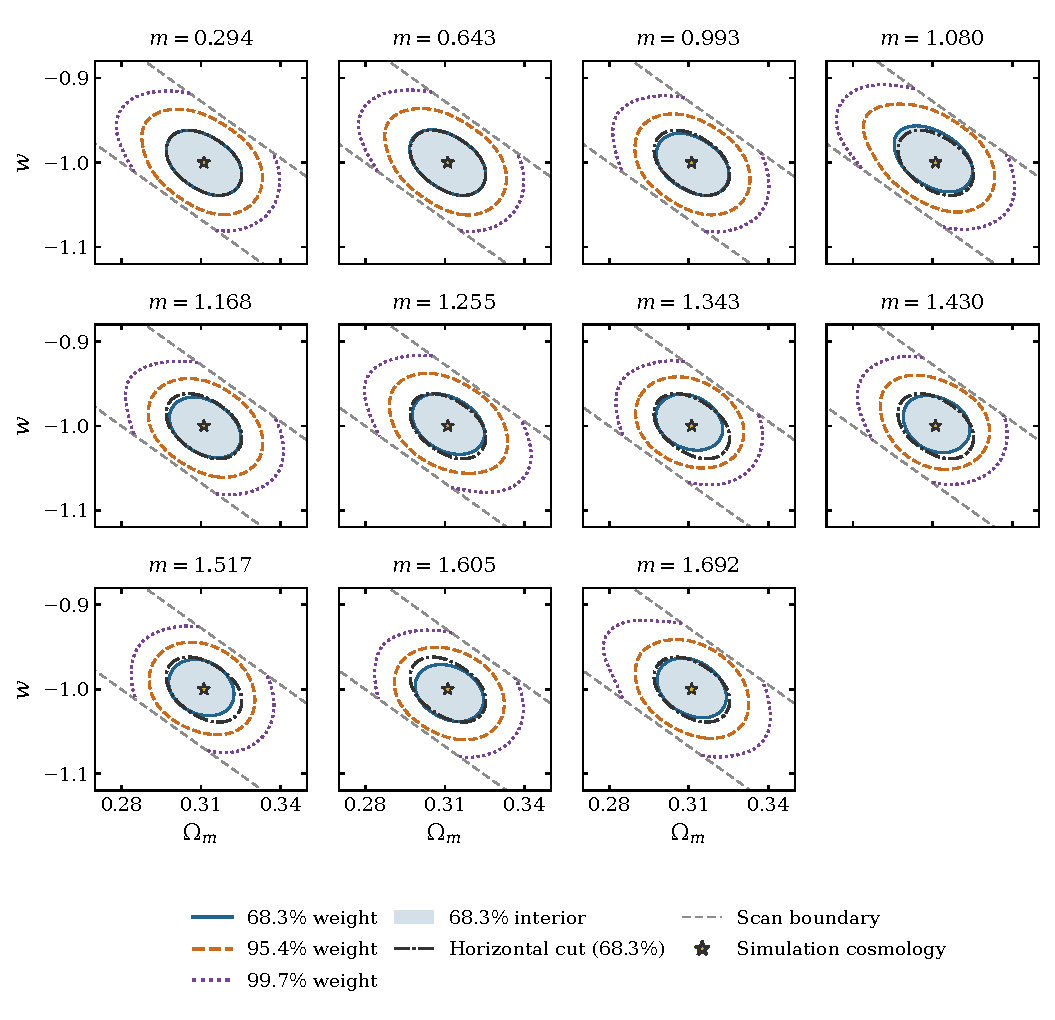
\includegraphics[width=.92\textwidth,height=.83\textheight,keepaspectratio]{figures/fig__intrinsic_subtracted_contours__eleven_m_smoothed.pdf}
\caption{All eleven wedge slopes. The dark dash-dotted curve gives the horizontal-cut 68.3 per cent reference. Other line styles, shading, boundary and star conventions follow Fig.~S2.}
\end{suppfigure}
\clearpage
\begin{suppfigure}
\centering
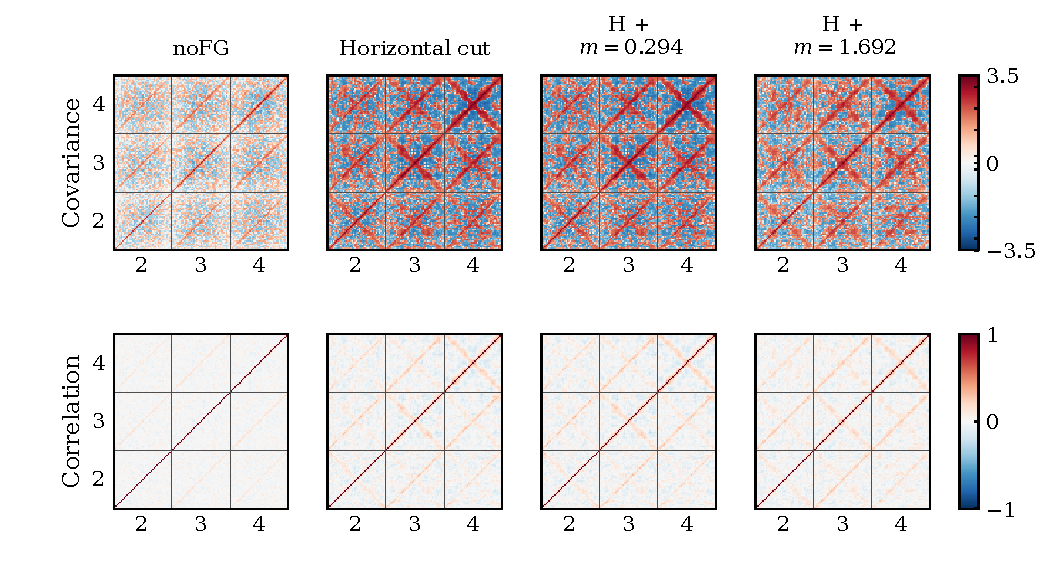
\includegraphics[width=.92\textwidth]{figures/fig__covmat.pdf}
\caption{Full regularized covariance (top, symmetric-logarithmic scale in $10^{-15}h^6\mathrm{Mpc}^{-6}$) and correlation matrices (bottom). Axis numbers identify the three redshift pairs; thresholds increase within each block. The covariance amplitudes complement the correlation-only main figure.}
\end{suppfigure}
\bigskip
\begin{supptable}
\centering
\caption{Joint areas and area ratios for the adopted smoothed weights. $A_{0.683}$ is in units of $10^{-4}$; each $\mathcal R_f$ is relative to the horizontal cut at the same weight fraction. All eleven wedge cases are retained. Areas remain conditional on the common finite scan domain; boundary contact is recorded in the accompanying CSV tables.}
\label{tab:sareas}
\begin{tabular}{@{}lrrrr@{}}
\toprule
Filter or $m$ & $A_{0.683}$ & $\mathcal R_{0.683}$ & $\mathcal R_{0.954}$ & $\mathcal R_{0.997}$ \\
\midrule
noFG & 59.56 & 3.807 & 3.955$^\dagger$ & 3.710$^\dagger$ \\
Horizontal & 15.65 & 1.000 & 1.000 & 1.000$^\dagger$ \\
0.294 & 15.65 & 1.000 & 1.000 & 1.000$^\dagger$ \\
0.643 & 15.83 & 1.012 & 1.012 & 1.015 \\
0.993 & 14.69 & 0.939 & 0.937 & 0.957 \\
1.080 & 16.45 & 1.052 & 1.083 & 1.094 \\
1.168 & 14.29 & 0.913 & 0.917 & 0.958 \\
1.255 & 14.51 & 0.927 & 0.960 & 1.010 \\
1.343 & 12.79 & 0.818 & 0.825 & 0.856 \\
1.430 & 13.03 & 0.833 & 0.855 & 0.881 \\
1.517 & 12.63 & 0.807 & 0.822 & 0.849 \\
1.605 & 13.16 & 0.841 & 0.846 & 0.881 \\
1.692 & 13.90 & 0.888 & 0.924 & 1.011$^\dagger$ \\
\bottomrule
\end{tabular}
\par\smallskip\begin{minipage}{.95\textwidth}\small
$\dagger$ Explicit boundary-contact flags in the four-treatment comparison indicate that these regions touch the scan hull. Flags for the remaining wedge slopes were not recorded in that comparison; their unmarked entries do not establish absence of boundary contact. All areas use the same finite integration domain.
\end{minipage}
\end{supptable}
\end{document}
